\chapter{Fundamentos teóricos}
\thispagestyle{empty}

\section{Aprendizaje automático}
El aprendizaje automático (Machine Learning, ML) \cite{20,21} es una rama de la IA y de las ciencias de la computación centrada en el uso de datos y algoritmos para imitar la forma en la que los humanos aprenden, detectando patrones o regularidades para realizar predicciones.

Existen 3 tipos de aprendizaje dentro del ML \cite{22,23}:

El \textbf{aprendizaje supervisado} consiste en entrenar con datos de los que se saben sus etiquetas (una etiqueta nos indica qué es cada dato). Por ejemplo, los datos de entrada podrían ser imágenes de animales y sus etiquetas podrían ser "perro" o "gato". A partir de los datos y sus etiquetas, el agente aprende una función que dado un nuevo dato, predice su etiqueta. Es el tipo de aprendizaje más utilizado, los datos vienen ya 'preparados' para su uso. Es el tipo de aprendizaje que utilizaremos en este TFG.

En el \textbf{aprendizaje no supervisado} el agente aprende los patrones de los datos de entrada sin ninguna realimentación, es decir, los datos no están etiquetados. La herramienta más usada en el aprendizaje no supervisado es el agrupamiento, que consiste en detectar potenciales grupos en los datos de entrada. Este enfoque requiere un mayor número de datos.

En el \textbf{aprendizaje por refuerzo} el agente aprende mediante una serie de recompensas o castigos. El agente intentará realizar acciones que le proporcionen mejores recompensas en el futuro. Este tipo de aprendizaje es muy utilizado para enseñar a jugar a juegos.

\section{Aprendizaje profundo}

\subsection{Redes neuronales}
Las redes neuronales (ANNs) \cite{24, 25, 27} son redes computacionales que intentan, a groso modo, simular el proceso de decisión de las neuronas del sistema nervioso central de los animales o humanos. Las ANNs poseen unidades de procesamiento de información llamadas neuronas, que están conectadas entre sí mediante capas. La red se compone de (ver Figura \ref{fig3}):
\begin{itemize}
	\item Una capa de entrada, que tendrá tantos inputs como características o variables tenga el problema
	\item Una o varias capas ocultas, compuestas por neuronas. El número de capas ocultas define la profundidad de la red neuronal.
	\item Una capa de salida, que representa el valor o valores predichos
\end{itemize} 

\begin{figure}[h]
	\centering
	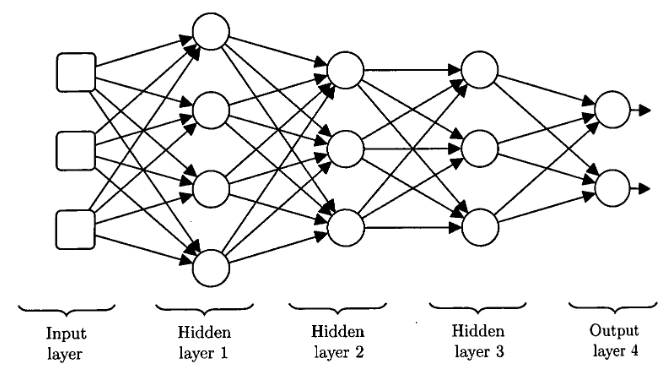
\includegraphics[scale=0.5]{imagenes/cap2/neural-network.png}
	\caption{Esquema de una red neuronal \cite{26}.}
	\label{fig3}
\end{figure}

Las neuronas son la unidad fundamental de cómputo, tienen varios valores de entrada y un valor de salida que se conecta con las neuronas de la siguiente capa. Los elementos básicos del modelo neuronal son (ver Figura \ref{fig4}):

\begin{itemize}
	\item Un conjunto de conexiones con las señales de entrada. Cada conexión tiene su propio peso/fuerza.
	\item Una función de suma de las señales de entrada, ponderadas cada una con su peso. Estas operaciones constituyen una combinación lineal.
	\item Una función de activación, para limitar la amplitud de la salida de la neurona. Normalmente, el rango de salida está en el intervalo [0,1], o alternativamente en [-1,1]. Existen muchos tipos de funciones de activación pero, se suelen utilizar cuatro: la función signo, la función logística, la función arco-tangente y la función ReLU.
\end{itemize} 

\begin{figure}[h]
	\centering
	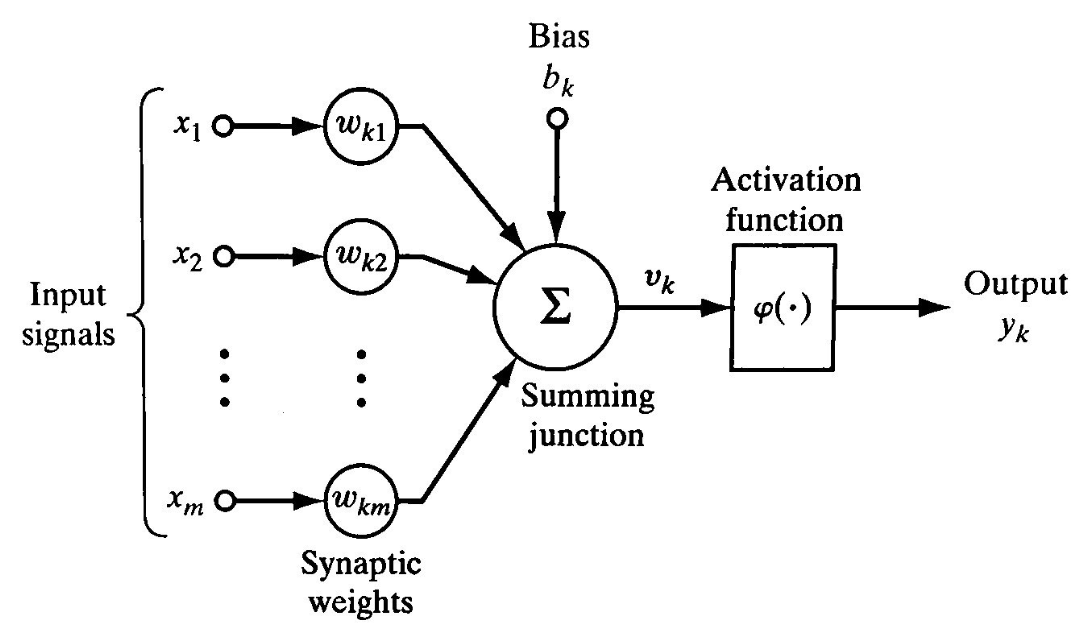
\includegraphics[scale=0.25]{imagenes/cap2/neuron-model.png}
	\caption{Modelo neuronal para una neurona $k$ \cite{25}.}
	\label{fig4}
\end{figure}

En términos matemáticos, podemos describir la salida de una neurona como:

\begin{equation}
	y = \phi(\sum_{j=1}^{m} w_j x_j + b)
\end{equation}

siendo $\phi$ la función de activación, $m$ el número de señales de entrada, $w_j$ el peso de cada entrada $x_j$, y $b$ el sesgo.

El algoritmo de aprendizaje de la red neuronal consiste en ir modificando los pesos y el sesgo, iterativamente, hasta alcanzar el resultado deseado. Este proceso iterativo se conoce como entrenamiento, y permite, a través de las modificaciones de los pesos, reconocer y extraer las características más relevantes de los datos.

El objetivo del entrenamiento es minimizar el error de predicción de la salida de la red neuronal, para ello, se define una función de pérdida. Existen numerosas funciones de pérdida, algunas de las más conocidas son: el error cuadrático medio (MSE), el error absoluto medio (MAE) o la entropía cruzada. La información de la función de pérdida se transmite desde la salida a la capa inicial, con el fin de adecuadamente los pesos para generar una mejor estimación de la predicción.

El sobreentrenamiento es un factor importante a evitar. Sobreentrenar el modelo de aprendizaje, significa, ajustarlo demasiado al conjunto de datos de entrenamiento, de manera que, al recibir nuevos datos no utilizados para entrenar, se estime un mal resultado debido a la poca capacidad de generalización ante nuevos datos.


\subsection{Redes neuronales convolucionales}
Las Redes Neuronales Convolucionales (Convolutional Neural Network, CNN) \cite{35, 36, 37} son un tipo de red neuronal profunda que trabaja con patrones de cuadrícula, como pueden ser imágenes (ver Figura \ref{fig5}).

Este tipo de redes neuronales incluyen dos tipos de capas adicionales: capas convolucionales y capas de pooling. Estas capas están en la primera parte de la red y son las encargadas de extraer las características relevantes de la entrada. Esto nos permite automatizar el proceso de extracción de características, a la vez que mejorarlo tanto en tiempo como en rendimiento.

\begin{figure}[h]
	\centering
	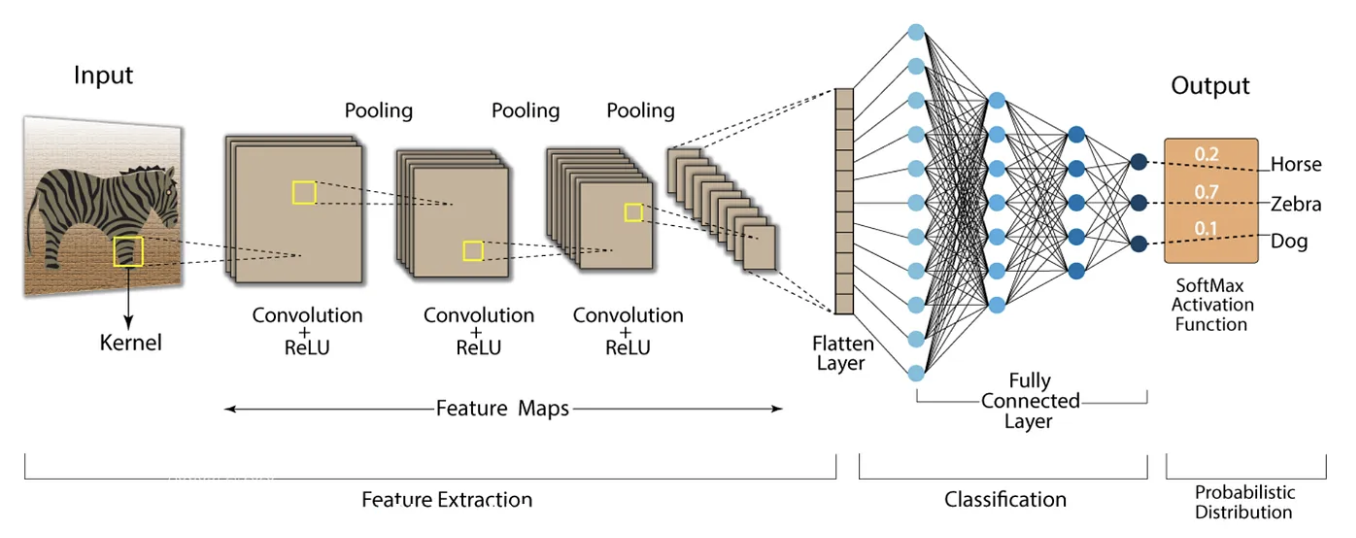
\includegraphics[scale=0.55]{imagenes/cap2/cnn.png}
	\caption{Ejemplo de CNN \cite{41}.}
	\label{fig5}
\end{figure}

A continuación, se describen los posibles tipos de capas presentes en una CNN \cite{39,40}:


\subsubsection*{Capa de convolución}

La capa convolucional es un componente fundamental de las CNN que se utiliza para extraer características de una imagen o conjunto de datos. Funciona aplicando operaciones de convolución a través de un conjunto de filtros o kernels sobre la entrada para detectar patrones visuales o características específicas en los datos (ver Figura \ref{fig6}).

%En términos simples, la operación de convolución implica deslizar un pequeño filtro (kernel) sobre la entrada, multiplicando los valores del filtro por los valores correspondientes en la región de la entrada en la que se encuentra. Estos productos se suman para producir un único valor en la salida, que se conoce como mapa de características o feature map.
%Al aplicar múltiples filtros en paralelo, la capa convolucional puede detectar diferentes características en paralelo, como bordes, texturas o formas en una imagen. Además, al compartir los pesos de los filtros a lo largo de la entrada, se logra la propiedad de "weight sharing", lo que reduce la cantidad de parámetros entrenables y hace que la red sea más eficiente.
%En resumen, la capa convolucional es responsable de extraer características significativas de los datos de entrada mediante operaciones de convolución, lo que permite a la red aprender patrones visuales complejos y realizar tareas como clasificación, detección de objetos o segmentación de imágenes de manera efectiva.

\begin{figure}[h]
	\centering
	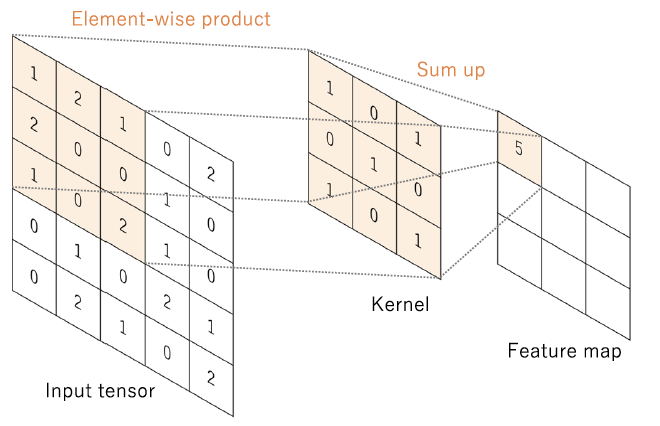
\includegraphics[scale=0.75]{imagenes/cap2/convolution.png}
	\caption{Ejemplo de convolución en CNN \cite{40}.}
	\label{fig6}
\end{figure}

Estos kernels pueden tener distintos tamaños y sus valores se aprenden a lo largo del entrenamiento de la red. Sin embargo, hay que tener en cuenta que la operación de convolución es lineal y no permite aprender patrones complejos. En este contexto es donde entra la capa de activación.

\subsubsection*{Capa de activación}

La capa de activación en una CNN sigue a la capa convolucional y se encarga de introducir no linealidades en el modelo mediante una función de activación.
Esta función aumenta la capacidad de la red para aprender relaciones no lineales en los datos, lo que es fundamental para capturar patrones más complejos. Algunas de las funciones de activación comunes utilizadas son la función ReLU (Rectified Linear Unit), la función sigmoide y la función tangente hiperbólica (ver Figura \ref{fig7}).

\begin{figure}[h]
	\centering
	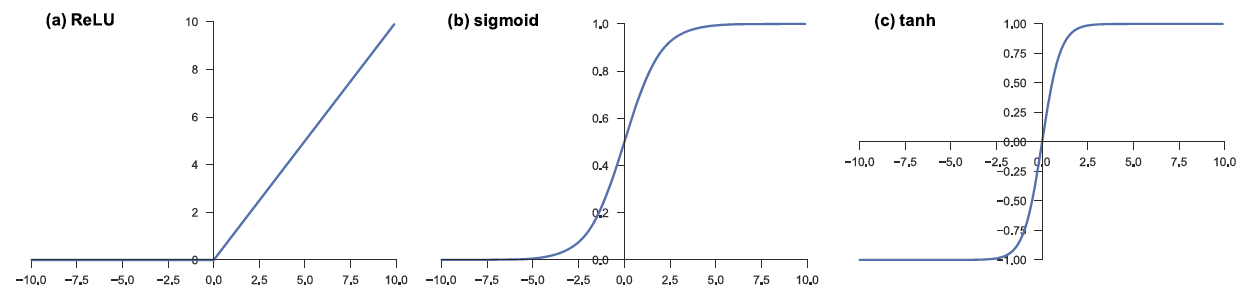
\includegraphics[scale=0.55]{imagenes/cap2/activation.png}
	\caption{Funciones de activación comúnmente aplicadas en CNN \cite{40}.}
	\label{fig7}
\end{figure}

\subsubsection*{Capa de pooling}
La capa de pooling también es específica de las CNN y se encarga de reducir la dimensionalidad de las características conservando la información más relevante.

Esta capa resume la información en regiones locales mediante una operación de downsampling en las características de entrada. Al reducir la dimensionalidad de las características, la capa de pooling disminuye el número de parámetros aprendibles en la red, lo que puede ayudar a prevenir el sobreajuste y mejorar la eficiencia computacional del modelo. Además, la capa de pooling también ayuda a introducir invariancia a pequeñas traslaciones y distorsiones en los datos de entrada, lo que permite a la red reconocer patrones incluso si están ligeramente desplazados en la imagen. 

Los dos tipos más comunes de pooling son el max pooling, que selecciona el valor máximo de una región local en las características de entrada, y el average pooling, que calcula el promedio de los valores en una región local (ver Figura \ref{fig8}).

\begin{figure}[h]
	\centering
	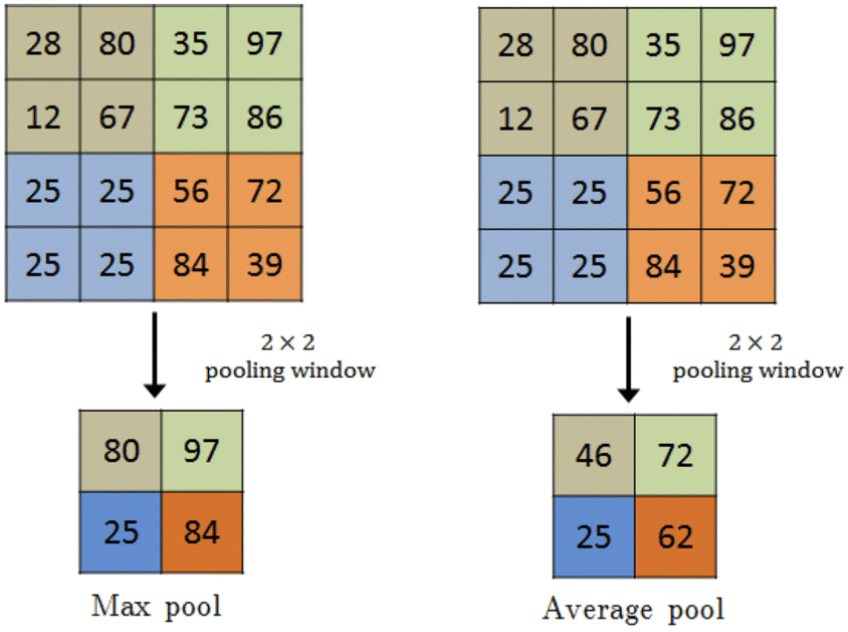
\includegraphics[scale=0.55]{imagenes/cap2/pooling.png}
	\caption{Tipos de pooling comúnmente utilizados en CNN \cite{40}.}
	\label{fig8}
\end{figure}

Los hiperparámetros de la capa de pooling incluyen el tamaño del filtro, el stride y el tipo de padding. Estos hiperparámetros afectan la forma en que se realiza el downsampling en las características.

% \subsubsection*{Capa de normalización}

\subsubsection*{Capa totalmente conectada}

La capa totalmente conectada sigue a las capas de convolución y pooling. En esta capa, las características extraídas por las capas anteriores se transforman en un formato unidimensional (vector) antes de conectarse a una o más capas totalmente conectadas, también conocidas como capas densas.

Esta capa, al igual que en las redes neuronales clásicas, tiene la responsabilidad de combinar y procesar las características extraídas para producir la salida final de la red.

Cada neurona en una capa totalmente conectada está conectada a todas las neuronas de la capa anterior a través de pesos aprendibles. Estos pesos determinan la contribución de cada neurona de entrada a la neurona de salida correspondiente en la capa totalmente conectada. Durante el entrenamiento, estos pesos se ajustan mediante algoritmos de optimización como backpropagation y descenso de gradiente para minimizar la diferencia entre las salidas predichas y las etiquetas reales.

Es importante destacar que la capa totalmente conectada suele estar seguida por una función de activación no lineal, como ReLU, para introducir no linealidades en el modelo y permitir la representación de patrones complejos en los datos. Además, la última capa de activación de la CNN, generalmente se selecciona según la naturaleza de la tarea que se está abordando.

\subsection{Transferencia de aprendizaje}

\section{Parámetros de la cámara y perspectiva}
	
\subsection*{Distancia cámara sujeto}

\subsection*{Longitud focal}
	
\subsection*{Distorsión de perspectiva}

